\documentclass{lab}

\renewcommand{\AA}{\ensuremath{\mathring{A}}}

\begin{document}

\labtitle{5.1.1}{Экспериментальная проверка уравнения Эйнштейна для фотоэффекта}{31~октября~2019~г.}{7~ноября~2019~г.}

\section*{Постановка эксперимента}

\begin{quote}
	\textbf{{\normalsize Цель работы: }}провести проверку уравнения Эйнштейна для фотоэффекта, определить экспериментально значение постоянной Планка.
\end{quote}

\begin{figure}[H]
	\centering
	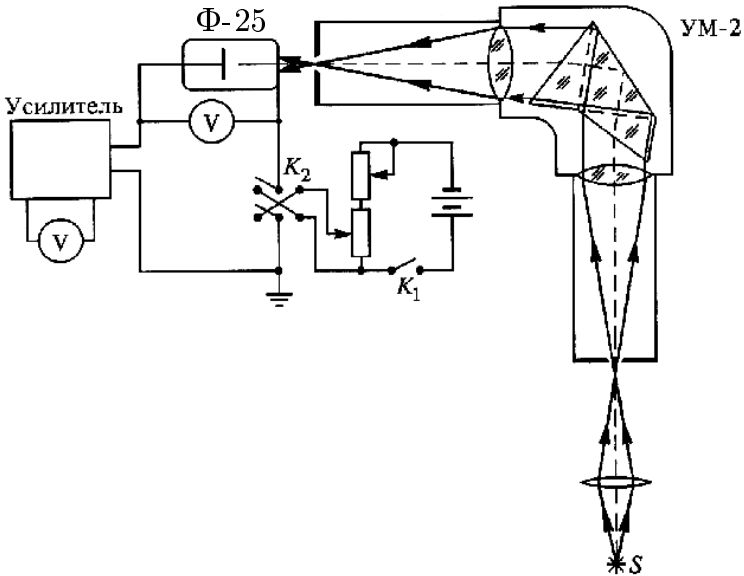
\includegraphics[width=0.65\linewidth]{scheme.png}
	\caption{Схема экспериментальной установки}
	\label{scheme1}
\end{figure}

%\begin{wrapfigure}[8]{r}{9cm}
%	\vspace{-0.3cm}
%	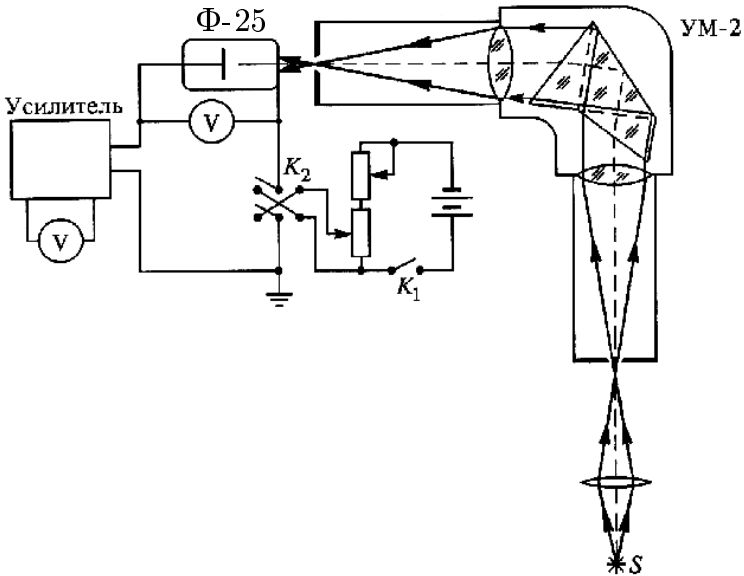
\includegraphics[width=9cm]{scheme.png}
%	\caption{Схема экспериментальной установки}
%	\label{scheme1}
%\end{wrapfigure}

Схема установки, используемой в работе, показана на рисунке \ref{scheme1}.

Приведем некоторые формулы, используемые в работе:
\begin{gather*}
\text{Энергетический баланс:}\\
\hbar\omega = E_{max} + W\\
\text{Запирающий потенциал:}\\
E_{max} = eV_0\\
eV_0 = \hbar\omega - W\\
\text{Наклон графика $V_0(\omega)$:}\\
\dfrac{dV_0}{d\omega} = \dfrac{\hbar}{e}
\end{gather*}

\section*{Выполнение работы}

Прокалибруем барабан монохроматора по спектру неоновой лампы, снимем зависимость фототока от потенциала катода для 6-8 длин волн в диапазоне 540-700 нм, по результатам измерений определим постоянную Планка и оценим работу выхода материала катода.

\begin{enumerate}
\item
Градуировка барабана монохроматора:

\begin{table}[H]
	\centering
	\begin{tabular}{|c|cccccc|}
		\hline
		$ \lambda,~\AA{} $ & 5400 & 5852 & 6143 & 6217 & 6402 & 6717 \\
		$ x,~дел $         & 2242 & 2502 & 2634 & 2694 & 2750 & 2865 \\ \hline
	\end{tabular}
	\caption{Градуировка}
	\label{tab1}
\end{table}

\begin{figure}[H]
	\centering
	\begin{tikzpicture}
	
	\pgfplotstableread{
		X	    Y		x-err	y-err
		2242	5400		20		90
		2502	5852		20		90
		2634	6143		20		90
		2694	6217		20		90
		2750	6402		20		90
		2865	6717		20		90
	}{\mytable}
	
	\begin{axis}[
	width = 0.8\textwidth,
	grid = major,
	xlabel = $ x\text{,~дел} $,
	ylabel = $ \lambda\text{,~\AA{}} $,
	ymin = 5200,
	ymax = 6800,
	xmin = 2200,
	xmax = 2900
	]

	
	\addplot[
	only marks,
	color = red,
	mark = *,
	error bars/.cd,
	x dir = both,
	x explicit,
	y dir = both,
	y explicit
	]
	table[
	x error = x-err,
	y error = y-err
	] {\mytable};
	
	\addplot[
	mark = none,
	color = red
	]
	table[
	y = {create col/linear regression={y=Y}}
	] % compute a linear regression from the
	{\mytable};
	
	\end{axis}
	\end{tikzpicture}
	\caption{$ y = 0.011x^2 - 3.7581x + 8072.8 $}
	\label{graph1}
\end{figure}

\item
Снимем зависимости тока от запирающего потенциала для разных частот:

\begin{table}[H]
	\centering \small
	\begin{tabular}{|c|cc|cc|cc|cc|cc|}
		\hline
		$ \lambda,~\AA{} $  & \multicolumn{2}{c|}{5400} & \multicolumn{2}{c|}{6717} & \multicolumn{2}{c|}{5852} & \multicolumn{2}{c|}{6143} & \multicolumn{2}{c|}{6402} \\
		$ x,~дел $          & \multicolumn{2}{c|}{2242} & \multicolumn{2}{c|}{2865} & \multicolumn{2}{c|}{2502} & \multicolumn{2}{c|}{2634} & \multicolumn{2}{c|}{2750} \\ \hline
		& $ U_{зап} $ & $ U_{фототок} $ & $ U_{зап} $ & $ U_{фототок} $ & $ U_{зап} $ & $ U_{фототок} $ & $ U_{зап} $ & $ U_{фототок} $ & $ U_{зап} $ & $ U_{фототок} $\\
		&5,37	&0,550	&5,42	&0,598	&5,41	&0,569	&5,426	&0,579	&5,42	&0,589\\
		&5,05	&0,544	&5,09	&0,594	&4,99	&0,564	&4,771	&0,572	&4,97	&0,583\\
		&4,49	&0,538	&4,55	&0,587	&4,43	&0,557	&4,087	&0,564	&4,51	&0,578\\
		&3,95	&0,529	&4,00	&0,578	&4,00	&0,551	&3,546	&0,555	&3,95	&0,573\\
		&3,52	&0,520	&3,51	&0,560	&3,55	&0,544	&2,998	&0,545	&3,43	&0,561\\
		&2,94	&0,508	&3,04	&0,559	&3,09	&0,536	&2,554	&0,534	&2,71	&0,545\\
		&2,01	&0,479	&2,42	&0,542	&2,45	&0,521	&1,960	&0,515	&2,08	&0,526\\
		&1,05	&0,409	&1,94	&0,523	&1,95	&0,504	&1,373	&0,489	&1,29	&0,486\\
		&0,39	&0,172	&1,32	&0,484	&1,48	&0,486	&1,036	&0,465	&0,72	&0,427\\
		&0,07	&0,137	&0,63	&0,380	&0,87	&0,437	&0,704	&0,425	&0,35	&0,186\\
		&-0,05	&0,112	&0,43	&0,298	&0,35	&0,325	&0,360	&0,334	&-0,03	&0,058\\
		&-0,12	&0,086	&0,33	&0,254	&-0,03	&0,125	&0,026	&0,159	&-0,20	&0,000\\
		&-0,18	&0,069	&0,18	&0,173	&-0,35	&0,000	&-0,044	&0,090	&-0,51	&-0,104\\
		&-0,30	&0,029	&0,02	&0,088	&-0,97	&-0,175	&-0,290	&-0,050	&-0,78	&-0,197\\
		&-0,40	&0,000	&-0,15	&0,000	&-1,45	&-0,338	&-0,492	&-0,172	&-1,06	&-0,291\\ \hline
		
	\end{tabular}
	\label{tab2}
\end{table}

\newpage

\item
Для каждой длины волны линеаризуем зависимость $ U_{фототок}(U_{зап}) $. Для этого построим графики $ \sqrt{U_{фототок}}(U_{зап}) $. Для каждого найдем коэффициенты уравнения прямой: $ y = ax + b $, затем коэффициент наклона $ b/a $. Результаты внесем в таблицу:

\begin{table}[H]
	\centering
	\begin{tabular}{|c|ccccc|}
		\hline
		$ \lambda,~\AA{} $         & 5852 & 6143 & 5400 & 6402 & 6717 \\
		$ V_0 = b/a,~В $           & 1.199 & 0.949 & 0.875 & 0.554 & 0.449 \\
		$ \omega,~10^{15}~с^{-1} $ & 3.22 & 3.07 & 3.49 & 2.94 & 2.80 \\
		\hline
	\end{tabular}
	\label{tab3}
\end{table}

\begin{figure}[H]
	\centering
	\begin{tikzpicture}
	
	\pgfplotstableread{
		X	    Y		x-err	y-err
		3.49	0.875		0.07		0.05
		2.94	0.554		0.07		0.05
		2.80	0.449		0.07		0.05
	}{\mytable}
	
	\begin{axis}[
	width = 0.8\textwidth,
	grid = major,
	xlabel = $ \omega $,
	ylabel = $ V_0 $,
	ymin = 0.4,
	ymax = 1,
	xmin = 2.6,
	xmax = 3.6
	]
	
	
	\addplot[
	only marks,
	color = red,
	mark = *,
	error bars/.cd,
	x dir = both,
	x explicit,
	y dir = both,
	y explicit
	]
	table[
	x error = x-err,
	y error = y-err
	] {\mytable};
	
	\addplot[
	mark = none,
	color = red
	]
	table[
	y = {create col/linear regression={y=Y}}
	] % compute a linear regression from the
	{\mytable};
	
	\end{axis}
	\end{tikzpicture}
	\caption{$ y = 0.6139x - 1.264 $}
	\label{graph2}
\end{figure}






\end{enumerate}

\subsection*{Итоги}
Исследовали фотоэффект, проверили формулу Эйнштейна.
По наклону графика определили постоянную Планка $ \hbar = 0.99 \cdot 10^{-34}~Дж \cdot с $.

\end{document}